%%%%%%%%%%%%%%%%%%%%%%%%%%%%% Define Article %%%%%%%%%%%%%%%%%%%%%%%%%%%%%%%%%%
\documentclass{article}
%%%%%%%%%%%%%%%%%%%%%%%%%%%%%%%%%%%%%%%%%%%%%%%%%%%%%%%%%%%%%%%%%%%%%%%%%%%%%%%

%%%%%%%%%%%%%%%%%%%%%%%%%%%%% Using Packages %%%%%%%%%%%%%%%%%%%%%%%%%%%%%%%%%%
\usepackage{geometry}
\usepackage{graphicx}
\usepackage{amssymb}
\usepackage{amsmath}
\usepackage{amsthm}
\usepackage{empheq}
\usepackage{mdframed}
\usepackage{booktabs}
\usepackage{lipsum}
\usepackage{graphicx}
\usepackage{color}
\usepackage{psfrag}
\usepackage{pgfplots}
\usepackage{bm}
\usepackage[hidelinks]{hyperref}
 \hypersetup{
   linktoc=all,
 }
%%%%%%%%%%%%%%%%%%%%%%%%%%%%%%%%%%%%%%%%%%%%%%%%%%%%%%%%%%%%%%%%%%%%%%%%%%%%%%%

% Other Settings

%%%%%%%%%%%%%%%%%%%%%%%%%% Page Setting %%%%%%%%%%%%%%%%%%%%%%%%%%%%%%%%%%%%%%%
\geometry{a4paper}

%%%%%%%%%%%%%%%%%%%%%%%%%% Define some useful colors %%%%%%%%%%%%%%%%%%%%%%%%%%
\definecolor{ocre}{RGB}{243,102,25}
\definecolor{mygray}{RGB}{243,243,244}
\definecolor{deepGreen}{RGB}{26,111,0}
\definecolor{shallowGreen}{RGB}{235,255,255}
\definecolor{deepBlue}{RGB}{61,124,222}
\definecolor{shallowBlue}{RGB}{235,249,255}
%%%%%%%%%%%%%%%%%%%%%%%%%%%%%%%%%%%%%%%%%%%%%%%%%%%%%%%%%%%%%%%%%%%%%%%%%%%%%%%

%%%%%%%%%%%%%%%%%%%%%%%%%% Define an orangebox command %%%%%%%%%%%%%%%%%%%%%%%%
\newcommand\orangebox[1]{\fcolorbox{ocre}{mygray}{\hspace{1em}#1\hspace{1em}}}
%%%%%%%%%%%%%%%%%%%%%%%%%%%%%%%%%%%%%%%%%%%%%%%%%%%%%%%%%%%%%%%%%%%%%%%%%%%%%%%

%%%%%%%%%%%%%%%%%%%%%%%%%%%% English Environments %%%%%%%%%%%%%%%%%%%%%%%%%%%%%
\newtheoremstyle{mytheoremstyle}{3pt}{3pt}{\normalfont}{0cm}{\rmfamily\bfseries}{}{1em}{{\color{black}\thmname{#1}~\thmnumber{#2}}\thmnote{\,--\,#3}}
\newtheoremstyle{myproblemstyle}{3pt}{3pt}{\normalfont}{0cm}{\rmfamily\bfseries}{}{1em}{{\color{black}\thmname{#1}~\thmnumber{#2}}\thmnote{\,--\,#3}}
\theoremstyle{mytheoremstyle}
\newmdtheoremenv[linewidth=1pt,backgroundcolor=shallowGreen,linecolor=deepGreen,leftmargin=0pt,innerleftmargin=20pt,innerrightmargin=20pt,]{theorem}{Theorem}[section]
\theoremstyle{mytheoremstyle}
\newmdtheoremenv[linewidth=1pt,backgroundcolor=shallowBlue,linecolor=deepBlue,leftmargin=0pt,innerleftmargin=20pt,innerrightmargin=20pt,]{definition}{Definition}[section]
\theoremstyle{myproblemstyle}
\newmdtheoremenv[linecolor=black,leftmargin=0pt,innerleftmargin=10pt,innerrightmargin=10pt,]{problem}{Problem}[section]
%%%%%%%%%%%%%%%%%%%%%%%%%%%%%%%%%%%%%%%%%%%%%%%%%%%%%%%%%%%%%%%%%%%%%%%%%%%%%%%

%%%%%%%%%%%%%%%%%%%%%%%%%%%%%%% Plotting Settings %%%%%%%%%%%%%%%%%%%%%%%%%%%%%
\usepgfplotslibrary{colorbrewer}
\pgfplotsset{width=8cm,compat=1.9}
%%%%%%%%%%%%%%%%%%%%%%%%%%%%%%%%%%%%%%%%%%%%%%%%%%%%%%%%%%%%%%%%%%%%%%%%%%%%%%%

%%%%%%%%%%%%%%%%%%%%%%%%%%%%%%% Title & Author %%%%%%%%%%%%%%%%%%%%%%%%%%%%%%%%
\title{Social A-S APP}
\author{Andrea Apicella - Giuseppe Squitieri}
%%%%%%%%%%%%%%%%%%%%%%%%%%%%%%%%%%%%%%%%%%%%%%%%%%%%%%%%%%%%%%%%%%%%%%%%%%%%%%%

\begin{document}
    \maketitle

    \tableofcontents

    \newpage

    \section{Area Utente}
    \subsection{Introduzione}
    L'area utente rappresenta il nucleo dell'applicazione, permettendo l'autenticazione sicura degli utenti registrati e l'accesso alle funzionalità principali del sito.

    \subsection{Registrazione}
    Gli utenti possono registrarsi tramite una pagina dedicata (\texttt{register.php}) inserendo:
    \begin{itemize}
        \item \textbf{Username} (univoco)
        \item \textbf{Password} (criptata tramite \texttt{password\_hash})
    \end{itemize}
    Il sistema verifica che l'username non sia già presente nel database prima di creare un nuovo account. I dati vengono salvati nella tabella \texttt{users}.

    \subsection{Login}
    L'autenticazione avviene tramite la pagina \texttt{login.php}, dove l'utente inserisce le proprie credenziali:
    \begin{itemize}
        \item Il sistema verifica l’esistenza dell’utente nel database.
        \item Se l’utente esiste, la password viene verificata con \texttt{password\_verify}.
        \item In caso di successo, viene creata una sessione contenente \texttt{\$ \_SESSION['username']} e \texttt{\$ \_SESSION['user\_id']}.
    \end{itemize}

    \subsection{Logout}
    La pagina \texttt{logout.php} consente all’utente di uscire dalla propria sessione. Il logout:
    \begin{itemize}
        \item Distrugge tutte le variabili di sessione attive.
        \item Reindirizza l’utente alla pagina di login.
    \end{itemize}

    \subsection{Home Page}
      Una volta loggato, l'utente può accedere alla home page, che presenta due sezioni principali:
      \begin{itemize}
        \item Creazione di un post: un form che consente all'utente di creare un post con un titolo (max 50 char), il contenuto (max 200 char),
          selezionare un colore per personalizzare il bordo del post.
          Il form invia dati tramite POST, che vengono salvati nel database nella tabella posts, assieme all'ID dell'utente che ha creato il post. Se titolo o contenuto sono vuoti, viene mostrato un errore.
        \item Nella colonna a destra della home vengono mostrati gli ultimi post con: titolo, nome autore, data di creazione,
          contenuto testuale, colore personalizzato.
          Questi sono ordinati dal più recente al più vecchio. Inoltre si può navigare tra questi post con degli appositi pulsanti (5 post per pagina).
      \end{itemize}

    \subsection{Navbar}
      La Navbar è inclusa in tutte le pagine, Contiene:
      \begin{itemize}
        \item Link alla home.
        \item Link alla pagina "About Us".
        \item Pulsante di logout.
        \item Link al Profilo.
      \end{itemize}

    \subsection{About Us}
      Pagina informativa sugli autori, con contenuti interattivi.


    \section{Modello dati}
      \begin{figure}[h!]
          \centering
          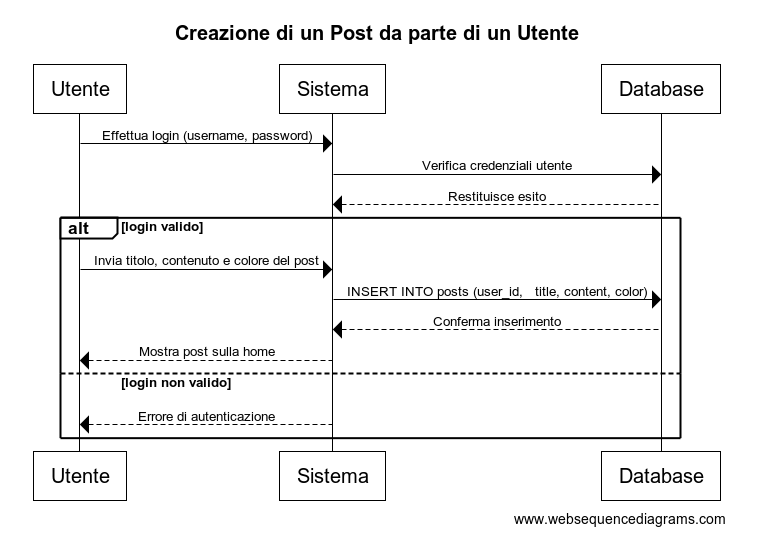
\includegraphics[width=0.8\textwidth]{Creazione.png}
          \caption{Diagramma UML delle tabelle Users e Posts}
          \label{fig:uml}
      \end{figure}

      \begin{figure}[h!]
          \centering
          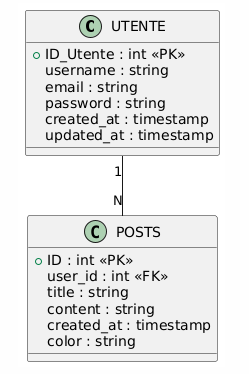
\includegraphics[width=0.4\textwidth]{ER.png}
          \caption{Tabella ER tabelle Users e Posts}
          \label{fig:er}

          \includegraphics[width=0.4\textwidth]{plantUML.png}
      \end{figure}


\end{document}

